\documentclass[11pt]{article}

% Packages
\usepackage[utf8]{inputenc}
\usepackage{amsmath}
\usepackage{amssymb}
\usepackage{graphicx}
\usepackage{hyperref}
\usepackage{amsthm}
\usepackage[margin=1in]{geometry}
\usepackage[numbers,sort&compress]{natbib}
\usepackage{listings}
\usepackage{algorithm}
\usepackage{algpseudocode}
\usepackage{tabularx}


% TikZ and diagram packages
\usepackage{tikz}
\usetikzlibrary{positioning,arrows,shapes,calc,decorations.pathreplacing}
\usepackage{forest}

% Theorem environments
\newtheorem{theorem}{Theorem}
\newtheorem{lemma}{Lemma}
\newtheorem{proposition}{Proposition}
\newtheorem{corollary}{Corollary}
\newtheorem{hypothesis}{Hypothesis}
\newtheorem{definition}{Definition}
\newtheorem{remark}{Remark}
\newtheorem{constraint}{Constraint}

% Paragraph formatting - no indentation, line breaks between paragraphs
\setlength{\parindent}{0pt}
\setlength{\parskip}{1em}

% Title and author
\title{Speed Without Waste: A Method-Centered Framework for Rapidly Generating Useful Outputs with Large Language Models}
\author{Author Name}
\date{\today}

\begin{document}

\maketitle
\begin{abstract}
Large language models (LLMs) are widely framed as creating a trade-off between speed and usefulness: faster interaction allegedly yields lower-quality outputs, while higher utility requires slower, expert-intensive refinement. This paper argues that “fast” and “useful” are not inherently in tension. The binding constraint is method. The pervasive problem is not that LLMs are intrinsically prone to low utility, but that common usage patterns systematically produce low-utility text—“junk”—through weak task specification, underspecified success criteria, minimal evaluation, and shallow iteration. We develop a theoretical framework explaining why junk is the default outcome under prevalent prompting habits: when goals are ambiguous, constraints are implicit, and feedback is absent or purely subjective, the model is optimized to generate plausible continuation rather than task-valid work, making fluent but non-actionable outputs a predictable equilibrium. Building on this account, the paper proposes a method-centered workflow—articulated as a small set of principles and a repeatable sequence of steps—for reliably producing useful outputs quickly. The workflow operationalizes utility as testable alignment with explicit requirements, emphasizes lightweight evaluation and structured iteration, and treats prompting as one component within a broader process of problem formulation, verification, and revision. The paper is conceptual and theoretical, offering no new empirical study, and contributes: (i) a clarified distinction between interaction speed and output utility, (ii) a causal account of how junk arises from method failures rather than model speed, (iii) an actionable methodology for rapid usefulness in routine LLM-supported tasks, and (iv) implications for LLM literacy, organizational adoption and governance, and research agendas focused on process design and evaluation.
\end{abstract}

\section{1. Problem Statement and Contribution Summary}

\subsection*{Cycle-time and usefulness objective under iterative prompting}
A minimal model distinguishing generation latency from end-to-end time-to-usable output, clarifying why speed-first prompting can increase total time and reduce expected utility, especially when evaluation is underspecified or informal (ref\_3) and when verification/mitigation steps for model errors (e.g., hallucinations) are omitted (ref\_1).

\begin{equation}
\label{eq:cycle_time}
T_{\mathrm{total}} \,=\, T_{\mathrm{gen}} \, + \, T_{\mathrm{eval}} \, + \, \sum_{i=1}^{K} \bigl(T_{\mathrm{reprompt}}^{(i)} + T_{\mathrm{fix}}^{(i)}\bigr),
\end{equation}

\begin{equation}
\label{eq:expected_utility}
\max_{\pi \in \Pi} \; \mathbb{E}\bigl[U(y\mid x,\mathcal{C})\bigr] \quad \text{s.t.} \quad \mathbb{E}\bigl[T_{\mathrm{total}}\bigr] \le \tau,
\end{equation}
where $x$ is the task input, $\mathcal{C}$ is the constraint set, $y$ is the final artifact, $K$ is the number of repair cycles induced by the interaction policy $\pi$, and $\tau$ is an available time budget.

\subsection*{Method beats speed-first prompting for time-to-usable outcomes}
A falsifiable statement that frames the paper’s argument—distinguishing interaction speed from output utility, attributing low-utility “junk” to method failures (e.g., weak specification, absent evaluation, shallow iteration), and motivating lightweight evaluation plus structured self-correction—while remaining within a non-experimental, theoretical contribution scope. (ref\_3) (ref\_4)

\begin{hypothesis}
\label{hyp:method_over_speed}
For a fixed model and task class, an interaction policy that (i) elicits constraints $\mathcal{C}$, (ii) introduces explicit grounding steps (e.g., retrieval when appropriate), and (iii) performs critique-and-revise before finalization yields (a) higher expected utility $\mathbb{E}[U(y\mid x,\mathcal{C})]$ and (b) no greater, and often lower, expected cycle time $\mathbb{E}[T_{\mathrm{total}}]$ than a speed-first policy that minimizes $T_{\mathrm{gen}}$ without structured evaluation.
\end{hypothesis}

Large language models (LLMs) are increasingly adopted as general-purpose cognitive tools for drafting, summarizing, planning, coding, and advising. Yet a recurrent phenomenon is observable across everyday professional and personal use: many users invoke LLMs primarily to obtain output quickly, then discover that the produced text is unusable (e.g., incorrect, insufficiently grounded, misaligned with constraints, or too generic to be operational). A common practical consequence is a loop of re-prompting, manual repair, and downstream verification that can erode---and in some cases negate---the time savings users sought. The broader consequence is that organizations and individuals may form inappropriate reliance patterns: over-trusting plausible content (a pattern documented in automation-bias studies in high-stakes human--AI decision-making) or, conversely, becoming overly skeptical after repeated low-utility outputs. \cite{ref_2}

We define and formalize this phenomenon as \emph{speed-first prompting}: an interaction style that optimizes for immediate linguistic fluency rather than decision-grade usefulness. Speed-first prompting is not simply ``bad prompting.'' It is a rational but incomplete adaptation to a tool that is fast, low-friction, and persuasive. Generative AI systems can increase throughput in workplace tasks, but benefits depend on how work is reorganized around the technology rather than on raw generation alone. \cite{ref_6} In this sense, the central failure mode is methodological: users conflate \emph{time-to-text} with \emph{time-to-usable-result}. The thesis of this paper is that speed and usefulness are not opposites; rather, usefulness emerges from method. In other words, the relevant optimization target is \emph{total cycle time} to a trustworthy, fit-for-purpose artifact, not the latency of the first draft.

To make this claim precise, we distinguish between (i) generation speed (how fast a model can produce tokens) and (ii) workflow efficiency (how fast a human--LLM system produces an acceptable outcome under constraints). Let $T_{\mathrm{gen}}$ denote time to generate an initial response, $T_{\mathrm{eval}}$ time to evaluate it, and $T_{\mathrm{fix}}$ time to correct or re-run. Under speed-first prompting, $T_{\mathrm{gen}}$ is minimized while $T_{\mathrm{eval}}$ and $T_{\mathrm{fix}}$ can inflate due to hallucinations, omissions, and mis-specified objectives. Hallucination remains a well-documented risk in LLM outputs, and survey work organizes mitigation techniques spanning prompting and decoding constraints, retrieval-based grounding, post-generation verification, and tool-augmented approaches. \cite{ref_1} Similarly, retrieval-augmented generation (RAG) is widely studied as an engineering pattern that conditions generation on retrieved documents to improve grounding and reduce unsupported claims, while also introducing retrieval- and evaluation-specific design challenges that must be managed. \cite{ref_5} These streams of work collectively imply that ``usefulness'' is not a property of the base model alone; it is a property of the interaction protocol and system architecture. \cite{ref_1,ref_5}

The problem is not merely inefficiency. When LLM outputs inform consequential judgments, the failure modes intersect with human decision biases. Evidence from human--AI decision-making research in high-stakes contexts shows that automation bias can bend decision processes toward deference to machine suggestions even when imperfections are known, and that reliance dynamics can also shift in the opposite direction when users disengage or discount the tool after negative experiences. \cite{ref_2} In everyday settings, analogous distortions arise when users accept persuasive but incorrect content, or when they repeatedly encounter low-utility generations and subsequently discount the tool even in contexts where it could help. Both outcomes degrade calibrated trust and can turn adoption into churn.

Accordingly, the paper addresses the following research question: \emph{How can practitioners systematically obtain fast \emph{and} usable LLM outputs without assuming new model capabilities or introducing proprietary evaluation infrastructure?} The approach is to provide (a) a theoretical framework that separates throughput from usefulness and (b) a practical methodology that operationalizes this separation into repeatable interaction patterns.

We define \emph{usefulness} as task-conditional fitness under constraints. Let $\mathcal{C}$ denote the set of explicit constraints (e.g., factual grounding, format, policy restrictions, scope, and audience), and let $U(y\mid x,\mathcal{C})$ denote the utility of output $y$ for input $x$ given constraints $\mathcal{C}$. The central claim is that method increases expected utility by eliciting missing constraints, forcing intermediate checks, and incorporating external grounding and critique where appropriate. Recent work on tool-interactive self-critique shows that structured critique-and-revision loops, especially when paired with external tools, can improve outputs by identifying and correcting errors across iterations, motivating a broader methodological stance: usefulness can be engineered via staged generation rather than hoped for in a single pass. \cite{ref_4}

This paper is intentionally scoped as a synthesis and formalization effort. It does not introduce new benchmarks, new evaluation metrics, or original experimental results. Instead, it translates established findings---hallucination mitigation surveys, RAG systematic reviews, self-correction via critique, and human evaluation best practices---into an integrated framework and an implementable workflow that prioritizes decision-grade outputs while preserving speed. \cite{ref_1,ref_3,ref_4,ref_5}

\paragraph{Contributions.} The paper makes four contributions.

\paragraph{(C1) Formal problem framing.} We formalize speed-first prompting as an optimization mismatch between minimizing $T_{\mathrm{gen}}$ and minimizing total cycle time to a usable artifact, and we provide a compact model linking iterative repair to expected utility.

\paragraph{(C2) Trust and decision-risk linkage.} We connect output unreliability to decision risk via known human factors, including automation bias, clarifying why ``plausible'' text is not a benign failure mode in applied settings. \cite{ref_2}

\paragraph{(C3) Methodology for fast usefulness.} We propose a practical, model-agnostic interaction methodology that uses constraint elicitation, grounding (including RAG when applicable), and critique-and-revise loops inspired by tool-interactive correction. \cite{ref_4,ref_5}

\paragraph{(C4) Evaluation boundary guidance.} Drawing on established guidance for human evaluation in NLP, we provide methodological boundaries for practitioners: what can be validated quickly by humans, what should be deferred to tools, and what requires domain oversight. \cite{ref_3}

\paragraph{Boundaries and non-contributions.} This paper does not claim new empirical performance improvements, does not introduce new automated metrics for truthfulness or usefulness, and does not evaluate systems in controlled user studies. It does not present organization-specific deployment case studies. Its purpose is to supply a rigorous conceptual map and a practical protocol that readers can adopt and, where needed, evaluate within their own settings.

\section{2. Conceptual Foundations: What Counts as ‘Useful’ vs ‘Junk’ Output?}

\subsection*{Multi-criteria usefulness functional}
Operational definition of task-relative usefulness as a weighted aggregation of six criteria, making utility explicit, testable, and evaluable via lightweight human evaluation and structured iteration (ref\_3), and supporting rapid refinement through critique-driven self-correction workflows (ref\_4).

\begin{equation}
\label{eq:usefulness}
U(y;\tau) \,=\, \sum_{k \in \{F,G,Co,S,A,V\}} w_k(\tau)\, s_k(y;\tau),
\qquad \sum_k w_k(\tau)=1,\quad w_k(\tau)\ge 0.
\end{equation}

\noindent where $s_F$ (fitness-for-purpose), $s_G$ (groundedness), $s_{Co}$ (correctness), $s_S$ (specificity), $s_A$ (actionability), and $s_V$ (verifiability) are criterion scores defined by the evaluation regime $E$ inside $\tau=\langle g,C,E\rangle$.

\subsection*{Conceptual taxonomy of usefulness vs junk output}
Criteria, positive definition, and corresponding junk failure mode(s) tied to weak task specification, underspecified success criteria, minimal evaluation, shallow iteration, and lack of verification/self-correction (ref\_3) (ref\_4). Include failure modes related to hallucination and mitigation-oriented criteria for usefulness (ref\_1), overreliance/automation bias as a pathway to accepting fluent but non-actionable outputs (ref\_2), and retrieval-grounding as a criterion to prevent ungrounded junk in knowledge-intensive tasks (ref\_5). Optionally connect to workplace productivity/quality outcomes when method improves useful outputs at speed (ref\_6).

\begin{table}[t]
\centering
\begin{tabular}{p{0.19\linewidth} p{0.40\linewidth} p{0.33\linewidth}}
\hline
\textbf{Criterion} & \textbf{`Useful' operationalization (task-relative)} & \textbf{Canonical `junk' failure mode(s)}\\
\hline
Fitness-for-purpose ($F$) & Advances goal $g$ while satisfying constraints $C$ & No decision value; misalignment with constraints \\
Groundedness ($G$) & Substantive claims supported by admissible sources under $E$ & Ungrounded claims; fabricated citations/details \\
Correctness ($Co$) & Claims are true/valid for the domain and task & Falsehoods; invalid reasoning; unfaithful summaries \\
Specificity ($S$) & Provides task-relevant precision (commits to concrete content when needed) & Genericity; excessive hedging; low information gain \\
Actionability ($A$) & Enables next steps/decisions consistent with $C$ & Vague advice; non-operational recommendations \\
Verifiability ($V$) & Checkable within bounded effort (sources, assumptions, traceability) & High checking cost; opaque assertions that invite over-trust \\
\hline
\end{tabular}
\caption{A criterion-level taxonomy linking useful properties to junk modes. Distinguishing criteria avoids collapsing safety-relevant issues (e.g., groundedness) into surface fluency.}
\label{tab:taxonomy}
\end{table}

\subsection*{Task-relative pathway from model output to perceived usefulness}
Minimal schematic showing how task definition and evaluation regime mediate usefulness judgments, emphasizing how weak specification and limited verification can yield fluent but non-actionable outputs and exacerbate automation bias effects (ref\_2). Highlights lightweight, structured evaluation practices (ref\_3) and iterative critique/self-correction workflows (ref\_4) as method-level interventions to improve reliability and reduce hallucination-driven failure modes (ref\_1).

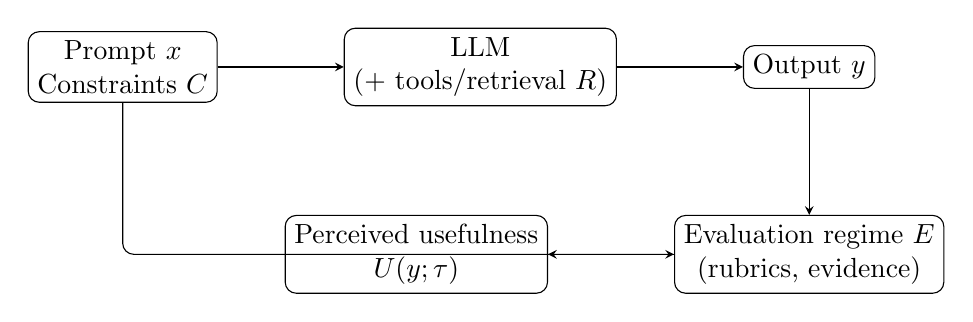
\begin{tikzpicture}[node distance=16mm,>=stealth,rounded corners]
\node (x) [draw,align=center] {Prompt $x$\\Constraints $C$};
\node (m) [draw,right=of x,align=center] {LLM\\(+ tools/retrieval $R$)};
\node (y) [draw,right=of m,align=center] {Output $y$};
\node (e) [draw,below=of y,align=center] {Evaluation regime $E$\\(rubrics, evidence)};
\node (u) [draw,left=of e,align=center] {Perceived usefulness\\$U(y;\tau)$};

\draw[->] (x) -- (m);
\draw[->] (m) -- (y);
\draw[->] (y) -- (e);
\draw[->] (e) -- (u);
\draw[->] (x) |- (e);
\end{tikzpicture}

\subsection*{Context dependence of usefulness judgments}
Non-quantitative, testable expectation aligning evaluation variation with observed disagreements in practice (ref\_3).

\begin{hypothesis}
\label{hyp:context}
For a fixed output $y$, perceived usefulness $U(y;\tau)$ will vary systematically with the task tuple $\tau=\langle g,C,E\rangle$, such that tightening constraints $C$ and increasing the cost of verification in $E$ (e.g., limited access to admissible evidence) increases the probability that fluent but ungrounded outputs are judged useful by non-expert evaluators, and judged junk by expert evaluators.
\end{hypothesis}

This paper requires an operational vocabulary for distinguishing outputs that create decision value from outputs that merely resemble competent language. Because large language models (LLMs) are general-purpose generators, ``usefulness'' cannot be treated as an intrinsic property of text; rather, it is a relation among an output, a task, a user, and an evaluation procedure. Accordingly, we define usefulness as a multi-criteria construct whose components correspond to what contemporary LLM safety and evaluation literatures treat as central risks (e.g., hallucination and over-trust) and practical mitigations (e.g., grounding, tool use, and human evaluation). \cite{ref_1,ref_2,ref_3,ref_4,ref_5}

\subsection{2.1 Formal object of evaluation}

Let a task be a tuple $\tau := \langle g, C, E \rangle$ where $g$ is the user goal (what the output is supposed to accomplish), $C$ is a set of constraints (format, scope, domain, policy, time, and resource constraints), and $E$ is an evaluation regime (the metrics, rubrics, adjudication processes, and permissible evidence). Let the model produce an output $y$ given prompt $x$ and (optionally) external resources $R$ such as retrieved documents or tools. Human evaluation guidance in NLP emphasizes that what counts as quality depends on study design choices---including constructs, task framing, and what annotators are asked to judge---thus $E$ must be specified rather than assumed. \cite{ref_3}

Under this framing, ``useful'' means ``fit for purpose under $\tau$,'' and ``junk'' means ``low or negative value under $\tau$,'' including cases where the output looks plausible but fails the relevant criteria (a risk emphasized by work on automation bias in high-stakes decision contexts). \cite{ref_2}

\subsection{2.2 Taxonomy of usefulness}

We operationalize usefulness via six criteria. These criteria are separable in principle and may trade off in practice, so evaluation should report them distinctly rather than collapsing into a single undifferentiated score.

\paragraph{(i) Fitness-for-purpose (goal satisfaction).}
An output is fit-for-purpose if it advances $g$ while satisfying $C$. This criterion is intentionally task-relative: the same text may be useful for brainstorming but junk for compliance documentation. In workplace deployments, value is often realized as time savings or improved task throughput; however, without assuming any specific numeric gains, the conceptual implication is that usefulness should be linked to workflow objectives, not only to linguistic quality. \cite{ref_6}

\paragraph{(ii) Groundedness (support in admissible sources).}
An output is grounded when its substantive claims are supported by admissible evidence under $E$ (e.g., retrieved documents in retrieval-augmented generation, cited policies, tool outputs). \cite{ref_5}
Hallucination surveys emphasize that ungrounded generations can be fluent yet unsupported, so groundedness must be evaluated explicitly (e.g., by checking whether substantive claims are backed by admissible sources) rather than inferred from style. \cite{ref_1}

\paragraph{(iii) Correctness (truth and validity).}
Correctness concerns whether claims about the world, the domain, or the task constraints are true or valid. Hallucination-mitigation literature distinguishes among factual errors, reasoning errors, and faithfulness errors; here, correctness is the umbrella notion that the output does not contain falsehoods or invalid inferences material to the task. \cite{ref_1}
Importantly, correctness is not always fully checkable in closed-book settings, motivating the need to assess verifiability as a separate dimension.

\paragraph{(iv) Specificity (task-relevant precision).}
Specificity captures whether an output commits to concrete, task-relevant content rather than generic phrasing. Generic outputs are often perceived as ``helpful'' at a glance but provide limited incremental information, especially to expert users. Specificity is context dependent: high-level summarization may be appropriately nonspecific, while procedural guidance should be concrete.

\paragraph{(v) Actionability (enables next steps).}
An output is actionable if it affords a clear next action or decision, consistent with $C$ (e.g., steps, options, checks, trade-offs). This criterion aligns with organizational uses of generative AI where utility arises from producing drafts, plans, or decision scaffolds. \cite{ref_6}
Actionability is not equivalent to correctness: an incorrect plan may be highly actionable yet harmful, which is why multi-criteria scoring is required.

\paragraph{(vi) Verifiability (checkability with bounded effort).}
Verifiability asks whether a user can efficiently determine groundedness and correctness. Outputs that make claims but omit sources, assumptions, or intermediate reasoning may impose high checking costs. Tool-interactive self-critique approaches and retrieval-augmented generation both implicitly target verifiability: retrieval makes supporting passages inspectable, while critique-and-revise loops iteratively surface weak claims and propose corrections that can then be checked. \cite{ref_4,ref_5}
In high-stakes environments where automation bias can cause humans to accept plausible outputs, verifiability becomes a safety-relevant component of usefulness. \cite{ref_2}

\subsection{2.3 Taxonomy of junk output}

Junk output is not merely ``low quality text.'' It is output that fails to produce decision value under $\tau$ or actively increases risk, cost, or confusion. We define five principal modes.

\paragraph{(a) Genericity (low information gain).}
Genericity is the failure mode where outputs remain at a level of abstraction that does not reduce uncertainty or progress the task. Genericity often co-occurs with hedging and platitudes; it can satisfy superficial fluency but not goal satisfaction.

\paragraph{(b) Ungrounded claims (hallucination/unsupported content).}
Ungroundedness arises when the model asserts facts, citations, or details not supported by admissible sources. Surveys of hallucination mitigation techniques treat this failure as central because fluent but unsupported content undermines calibrated trust and can propagate errors when reused in downstream artifacts and decisions. \cite{ref_1}

\paragraph{(c) Incoherence (internal inconsistency or non sequitur).}
Incoherence refers to contradictions within the output, broken logical relations, or content that does not follow from the prompt. Incoherence can be obvious (nonsensical text) or subtle (incompatible constraints).

\paragraph{(d) Misalignment with constraints.}
Even a correct and grounded answer can be junk if it violates constraints in $C$ (wrong format, disallowed content, exceeding scope, ignoring role or policy requirements). This mode matters because many real deployments are constraint-heavy (policy, privacy, domain restrictions).

\paragraph{(e) Lack of decision value (no effect on action under bounded resources).}
An output can be fluent, correct, and even grounded yet still not worth using if it does not change a decision or reduce effort relative to baselines. This is especially salient in professional settings: usefulness is ultimately comparative and opportunity-cost aware.

\subsection{2.4 A task-relative model of perceived usefulness}

Perceived usefulness depends on what users notice and what evaluators score. Human evaluation methodology emphasizes that measurement choices (construct definitions, rubrics, and study design) shape conclusions, while studies of automation bias show that humans may overweight system outputs---particularly when presented confidently or under procedural/time pressure that discourages independent checking. \cite{ref_2,ref_3}
Thus, two evaluators with different $E$ may disagree about whether the same output is useful.

To formalize this dependence, we treat usefulness as a weighted aggregation of criteria, where weights are induced by task demands and risk tolerance. Let $\mathcal{D}(y;\tau)$ denote decision value: the extent to which $y$ improves the expected quality, speed, or reliability of decisions under $\tau$. Then perceived usefulness is a function of both intrinsic properties of $y$ (groundedness, correctness, etc.) and extrinsic evaluation conditions (what evidence is available, what checking is feasible).

This framing yields two implications for the rest of the paper. First, evaluation must be criterion-explicit: a single headline score conflates orthogonal properties and obscures failure modes. Second, mitigation strategies should be mapped to criteria: retrieval-augmented generation primarily targets groundedness and verifiability; tool-interactive critique targets correctness and constraint adherence by iterative checking; and human evaluation protocols must align annotation rubrics with task goals. \cite{ref_3,ref_4,ref_5}

\subsection{2.5 Testable expectations (without new data)}

Because usefulness is task-relative, the same system may appear highly useful in low-stakes creative tasks yet junk in high-stakes analytic tasks, even when surface fluency is identical. Moreover, interventions that increase evidence visibility or structured critique should improve perceived usefulness primarily through groundedness and verifiability, while interventions that constrain generation (formats, guardrails) should reduce constraint-misalignment junk. \cite{ref_4,ref_5}
These expectations organize later empirical and design discussions without presuming any particular numeric effect sizes.

\section{3. Why ‘Junk’ is the Default: A Causal Model of Common LLM Misuse}

\subsection*{Causal diagram of default junk production}
A minimal causal graph linking underspecification, constraints, context, evaluation, and verification to junk output via both model and human factors pathways (ref\_2)(ref\_3)(ref\_1)(ref\_4).

\begin{tikzpicture}[node distance=14mm, >=Stealth, every node/.style={font=\small}]
  \node[draw, rounded corners, align=center] (G) {User goal $G$};
  \node[draw, rounded corners, right=of G, align=center] (P) {Prompt $P$};
  \node[draw, rounded corners, below=of P, align=center] (C) {Constraints $C$};
  \node[draw, rounded corners, right=of P, align=center] (K) {Context/Evidence $K$};
  \node[draw, rounded corners, right=of K, align=center] (Y) {LLM output $Y$};
  \node[draw, rounded corners, below=of Y, align=center] (E) {Evaluation rubric $E$};
  \node[draw, rounded corners, below=of K, align=center] (V) {Verification loop $V$};
  \node[draw, rounded corners, right=of Y, align=center] (J) {Junk $J$};
  \node[draw, rounded corners, below=of E, align=center] (A) {Automation bias};

  \draw[->] (G) -- (P);
  \draw[->] (C) -- (P);
  \draw[->] (P) -- (Y);
  \draw[->] (K) -- (Y);
  \draw[->] (Y) -- (J);
  \draw[->] (E) -- (J);
  \draw[->] (V) -- (J);
  \draw[->] (A) -- (E);
\end{tikzpicture}

\subsection*{Junk is a low-governance equilibrium}
A testable theoretical claim connecting specification, evaluation, and verification to junk prevalence independent of generation speed (ref\_3).

\begin{hypothesis}[Junk as a governance equilibrium]
Holding the base model $p_\theta$ fixed, the expected prevalence of junk output decreases as organizations increase (i) prompt--goal alignment, (ii) explicit constraint specification, (iii) grounding context availability, (iv) rubric-based evaluation, and (v) verification-loop strength. Conversely, increasing generation speed without strengthening (iv) and (v) does not reduce junk and can increase the rate at which unverified artifacts enter workflows.
\end{hypothesis}

The motivating observation for this section is that organizations can obtain fluent-looking text from large language models (LLMs) yet still encounter low downstream value, rework, or outright failure when outputs are not integrated into workflows with explicit checking and oversight. This is sometimes perceived as a speed problem (``the model is fast but unreliable''). A more accurate diagnosis is that junk output is a method and governance problem: absent a disciplined specification--evaluation--verification workflow, the default interaction mode invites the model to fill underspecified degrees of freedom with plausible continuations rather than warranted claims.

\subsection{A causal account of why junk appears by default}

Let an LLM be a conditional distribution over text sequences. Given an input prompt $x$ and previous tokens $y_{<t}$, the model generates the next token by
\begin{equation}
\label{eq:next-token}
\hat{y}_t \sim p_\theta(y_t \mid x, y_{<t}),
\end{equation}
with the full completion $\hat{y}$ produced by iterating this process. This next-token objective does not, by itself, encode truth, task success, domain compliance, or epistemic humility; it primarily encodes patterns of continuation that were rewarded during training. Consequently, when the prompt leaves key task variables unspecified, the model must still produce a completion; the induced behavior is not ``refusal'' but interpolation over likely continuations.

We formalize a minimal causal model for ``junk'' as output that is (i) misaligned with the user goal, (ii) unconstrained relative to domain or policy requirements, (iii) unverified, or (iv) evaluated against no explicit rubric. Let $G$ denote the (latent) user goal, $P$ the prompt actually provided, $C$ the set of constraints that would make a response acceptable, $K$ the relevant domain context/evidence available at generation time, $Y$ the model output, $E$ the evaluation procedure, and $V$ a verification loop (e.g., retrieval, tools, tests, or human checking). Let $J$ be an indicator of junk (with $J=1$ denoting junk).

Mechanistically, common misuse patterns map onto six failure channels:
\paragraph{(1) Underspecified prompts ($P \not\approx G$).} Users frequently provide prompts that omit purpose, audience, scope boundaries, assumptions, and desired level of rigor. Because the model must complete text regardless, it will select high-probability continuations that may be locally coherent yet globally wrong for the intended use.

\paragraph{(2) Missing constraints ($C$ absent from $P$).} Even when the goal is clear (e.g., ``draft a policy memo''), constraints such as citation requirements, allowed sources, prohibited claims, formatting, risk posture, and uncertainty handling are often omitted. Sensitivity to instructions implies that small changes in constraint phrasing can induce large changes in output; absent constraints, the model defaults to generic genre conventions.

\paragraph{(3) Absent evaluation rubrics ($E$ undefined or informal).} Without a rubric, ``quality'' collapses to surface fluency. Human evaluation in NLP emphasizes that evaluation requires explicit constructs, tasks, and measurement plans; otherwise, judgments become inconsistent and vulnerable to framing and rater biases. \cite{ref_3} If the only implicit metric is readability, the system will optimize for readability.

\paragraph{(4) Over-trust in fluent text (automation bias).} Fluent completions can trigger undue reliance, especially in high-stakes contexts. Work on automation bias in decision-making contexts shows that people can overweight machine outputs and shift toward deference, including in high-stakes settings where decision-makers are aware that the automated recommendations are imperfect. \cite{ref_2} When this bias co-occurs with weak evaluation and no verification, junk survives and propagates.

\paragraph{(5) Lack of domain context/evidence ($K$ missing).} The model cannot condition on facts not present in its context window and, without retrieval or tool use, cannot reliably ground claims in up-to-date or task-specific sources. Retrieval-augmented generation (RAG) is motivated precisely by this gap: augmenting $K$ with retrieved documents can improve grounding, but it introduces its own challenges---including retrieval errors, incomplete coverage, and the need to evaluate whether cited passages truly support the generated claims. \cite{ref_5}

\paragraph{(6) No verification loop ($V$ absent).} The decisive governance failure is treating the first completion as a deliverable rather than a draft to be stress-tested. Hallucination surveys emphasize that hallucination is more likely under uncertainty and weak grounding; correspondingly, common mitigation families rely on retrieval-based grounding, post-generation verification, structured self-critique, and external checks. \cite{ref_1} Tool-interactive critiquing methods such as CRITIC exemplify this principle: the model generates, critiques its own output, consults external tools, and revises across iterations, turning generation into a loop rather than a one-shot. \cite{ref_4}

\subsection{From mechanisms to an explicit risk model}

To make the above causal story operational, define a scalar ``specification-and-governance adequacy'' score $S \in [0,1]$ as a function of prompt completeness, constraint explicitness, available evidence/context, evaluation rubric clarity, and verification strength:
\begin{equation}
\label{eq:adequacy}
S \;=\; w_P s_P + w_C s_C + w_K s_K + w_E s_E + w_V s_V,\qquad \sum_i w_i = 1,\; w_i \ge 0.
\end{equation}
Here $s_P$ measures alignment between $P$ and $G$ (task specification), $s_C$ encodes constraint coverage, $s_K$ captures grounding context sufficiency (including retrieval/tool outputs), $s_E$ represents the presence of an explicit rubric and evaluation plan, and $s_V$ represents verification-loop strength. This is not presented as an empirically calibrated model; it is a conceptual device for reasoning about why ``junk'' occurs systematically.

We then posit that junk probability decreases monotonically with adequacy:
\begin{equation}
\label{eq:junkprob}
\Pr(J=1 \mid S) = \sigma(\alpha - \beta S), \qquad \beta > 0,
\end{equation}
where $\sigma$ is a logistic function, $\alpha$ captures baseline risk due to model limitations, and $\beta$ reflects the effectiveness of specification and governance.

This formulation highlights why speed is not the primary cause. Generation latency affects throughput, but the dominant determinant of junk is $S$: when $S$ is low, the model is effectively asked to (i) infer $G$, (ii) invent constraints, (iii) supply missing evidence, and (iv) grade itself with no rubric, all while being rewarded for fluent continuation.

\subsection{A compact causal graph}

The causal dependency can be summarized by: underspecification and missing constraints lower $S$; missing context increases uncertainty; automation bias reduces scrutiny; absent evaluation and verification prevent correction. This produces a stable failure mode: fluent text passes as ``done.''

\subsection{Hypothesis: junk as a governance equilibrium}

The above suggests a governance equilibrium: if organizational processes reward speed of drafting over correctness and auditability, interactions will converge to low $s_E$ and $s_V$, and thus high junk risk. Conversely, instituting explicit rubrics and verification loops should shift the equilibrium even with the same base model.

\subsection{Linking to known properties of LLMs}

The mechanisms above follow from well-known model properties:

\paragraph{Next-token prediction and underspecification.} Under Eq.~\eqref{eq:next-token}, the model is optimized to continue text plausibly; if a prompt fails to identify the decision boundary (what must be true, what is optional, what is unknown), the model will allocate probability mass to plausible but unwarranted specifics.

\paragraph{Hallucination under uncertainty.} When $K$ is thin and the prompt implicitly demands specificity, the model faces a trade-off: produce vague text (often judged unhelpful) or produce specific text (often judged helpful but more likely to be false). Hallucination mitigation surveys organize countermeasures around grounding, uncertainty estimation, post-hoc verification, and training-time interventions; the common theme is that hallucination is not merely ``random error'' but a predictable response to missing constraints and evidence. \cite{ref_1}

\paragraph{Instruction sensitivity and constraint omission.} Because LLM outputs shift meaningfully with changes to instructions, the absence of explicit constraints is itself an instruction: ``use generic priors.'' In governance terms, failure to specify constraints is equivalent to delegating policy to the model's training distribution.

\paragraph{Context limitations and domain mismatch.} Without retrieval or tools, $K$ is limited to what fits in context and what the model can internally recall. RAG addresses this by injecting retrieved documents into $K$, but systematic reviews of RAG emphasize that retrieval introduces new failure points: wrong retrieval, overreliance on retrieved snippets, and evaluation challenges. \cite{ref_5} Thus, adding context without governance (rubrics and verification) can still yield junk.

\paragraph{Automation bias and evaluation collapse.} Human factors research on automation bias indicates that people can defer to automated outputs even when those outputs warrant scrutiny, particularly when procedures do not enforce independent checking. \cite{ref_2} In LLM settings, fluency further increases perceived competence, making it easier for outputs to pass through without adversarial checking. This is a socio-technical amplifier: the model produces plausible continuations, and the human process treats plausibility as validity.

\paragraph{Verification loops as the missing control system.} Tool-interactive critiquing (e.g., CRITIC) provides a template for turning one-shot generation into a control loop: generate, critique, consult tools, revise. \cite{ref_4} The key governance insight is that verification cannot be a vague intention; it must be designed as a repeatable loop with stopping conditions and explicit failure handling.

\subsection{Implication: reduce junk by increasing adequacy, not by slowing down}

The causal model implies that reducing junk is primarily about increasing $S$ via method: richer specifications, explicit constraints, domain grounding, rubric-based evaluation, and verification loops. This reframes the productivity narrative common in workplace discussions of generative AI: speed may increase, but without a corresponding increase in evaluation and verification capacity, the organization can simply produce incorrect artifacts faster. \cite{ref_6} The central design problem is thus governance: deciding what must be specified, how it will be evaluated, and how claims will be verified before outputs are allowed to influence decisions.

\section{4. Core Thesis: Speed and Usefulness are Orthogonal Under a Method Lens}

\subsection*{Orthogonality as a two-stage generate--evaluate model}
Formalizes speed as an execution variable and usefulness as an evaluation functional applied to the produced artifact, aligning with structured evaluation practices in NLP and iterative critique/self-correction workflows for LLM outputs (ref\_3) (ref\_4).

\begin{equation}
\label{eq:gen-eval}
\underbrace{y \sim G_m(\cdot \mid x,c)}_{\text{execution (generation) under method } m},\qquad 
\underbrace{u = U(y; x,c)}_{\text{evaluation (usefulness) in context } c},\qquad 
\underbrace{T = T(m;x,c)}_{\text{execution time}}.
\end{equation}

\begin{equation}
\label{eq:accept}
\text{Accept}(y) \;\Longleftrightarrow\; U(y;x,c) \ge \tau(c),
\end{equation}

\subsection*{2×2 matrix: Fast/Slow × Useful/Junk}
A minimal conceptual diagram demonstrating that all four quadrants are logically possible, supporting the orthogonality claim (ref\_6).

\begin{figure}[t]
\centering
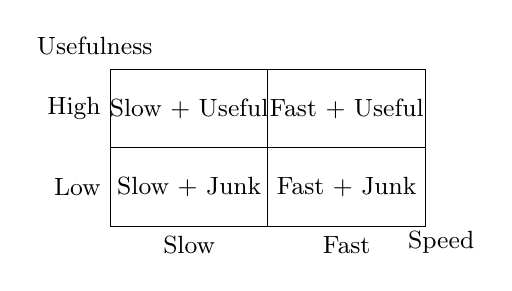
\begin{tikzpicture}[font=\small]
  % axes labels
  \node at (-0.2,2.3) {Usefulness};
  \node at (4.2,-0.2) {Speed};

  % grid
  \draw (0,0) rectangle (4,2);
  \draw (2,0) -- (2,2);
  \draw (0,1) -- (4,1);

  % quadrant labels
  \node at (1,1.5) {Slow + Useful};
  \node at (3,1.5) {Fast + Useful};
  \node at (1,0.5) {Slow + Junk};
  \node at (3,0.5) {Fast + Junk};

  % axis tick labels
  \node[anchor=east] at (0,1.5) {High};
  \node[anchor=east] at (0,0.5) {Low};
  \node[anchor=north] at (1,0) {Slow};
  \node[anchor=north] at (3,0) {Fast};
\end{tikzpicture}
\caption{Speed and usefulness are orthogonal dimensions under a method lens: each quadrant is feasible depending on specification and evaluation checks.}
\label{fig:2x2}
\end{figure}

\subsection*{Method-mediated shift from Fast+Junk to Fast+Useful}
A falsifiable hypothesis connecting method design—explicit task specification, lightweight evaluation, and structured self-correction checks—to expected usefulness at comparable speed (ref\_3) (ref\_4), mitigating fluent but non-actionable or error-prone outputs (ref\_1).

\begin{hypothesis}
\label{hyp:method}
For a fixed task context $c$ and input distribution over $x$, methods $m$ that (i) front-load explicit specifications of requirements and (ii) implement lightweight checks (e.g., retrieval grounding, critique, or human verification gates for high-risk contexts) yield higher expected usefulness $\mathbb{E}[U(y;x,c)]$ at comparable execution time $T(m;x,c)$ than ad hoc prompting methods lacking such evaluation linkages.
\end{hypothesis}

This section formalizes the paper's central claim: 
(i) \emph{speed} is primarily an \emph{execution} property of a generative pipeline (how quickly candidate outputs are produced), whereas 
(ii) \emph{usefulness} is primarily an \emph{evaluation} property (whether an output satisfies task-relevant criteria under a decision context). The common intuition that ``faster'' models are thereby ``more useful'' conflates these two axes. Under a method lens, the axes are orthogonal: one can generate quickly and still generate low-quality or unsafe content, or generate slowly and still fail to meet requirements. Conversely, speed and usefulness can co-exist when a method explicitly couples generation to specification and lightweight evaluation.

\subsection{Definitions: separating execution from evaluation}
Let a user-task context be denoted by $c$ (including domain, risk, audience, and constraints). A generative interaction produces an output $y$ in response to an input $x$ under some method $m$ (prompting style, tool use, retrieval, post-processing, checks). We define two distinct quantities.

First, define \emph{execution speed} as an operational property of the production pathway:
$T(m;x,c)$ is the time-to-candidate (or more generally, the time-to-accepted-output) induced by method $m$.

Second, define \emph{usefulness} via an evaluation functional $U$ that maps the produced output to a scalar (or vector) quality score given context:
$U(y; x,c)$. This explicitly separates the \emph{artifact} $y$ from the \emph{judgment} of that artifact under task requirements.

The distinction aligns with three empirical literatures. (1) Hallucination surveys emphasize that fluent outputs can be non-factual, misleading, or ungrounded without grounding and verification; correspondingly, mitigation families span constraint- and decoding-based controls, retrieval grounding, calibration, and post-hoc checking---i.e., augmenting evaluation and control rather than merely accelerating generation. \cite{ref_1} (2) Studies of automation bias show that users may over-trust machine recommendations, especially under time pressure or when procedures do not require independent checking; here, speed can \emph{increase} the risk of acceptance without evaluation. \cite{ref_2} (3) Human evaluation methodology in NLP highlights that ``quality'' is not a single intrinsic property but must be measured against clearly specified constructs and protocols, reinforcing usefulness as an evaluation concept rather than a timing artifact. \cite{ref_3}

\subsection{A conceptual model: a 2\,$\times$\,2 matrix of outcomes}
We can express the orthogonality claim with a minimal discrete model. Partition speed into \{Fast, Slow\} and usefulness into \{Useful, Junk\}. ``Junk'' denotes outputs that fail task criteria (incorrect, irrelevant, unsafe, unverifiable, or misaligned with constraints), even if linguistically fluent. ``Useful'' denotes outputs meeting an acceptable threshold under the evaluation functional.

This model implies all four quadrants are feasible:
(i) Fast+Useful: the desired regime; 
(ii) Fast+Junk: rapid but unvalidated content; 
(iii) Slow+Useful: careful but time-consuming workflows; 
(iv) Slow+Junk: wasted time with no value. 

Critically, typical ad hoc use of LLMs often drifts toward Fast+Junk, not because the model is intrinsically ``junk,'' but because the method omits specification (what counts as good) and evaluation (how we know it is good). In the absence of explicit constraints, the model optimizes for plausible continuation rather than task validity; in the absence of checks, users may accept plausible-but-wrong outputs, an effect consistent with automation bias in consequential domains. \cite{ref_2}

\subsection{Why method changes the quadrant: front-loading specification and lightweight checks}
Under a method lens, the question is not ``Is the model fast?'' but ``Does the method convert model speed into decision-relevant value?'' Two design moves shift mass from Fast+Junk to Fast+Useful.

\paragraph{Front-loading specification.}
Specification makes the evaluation functional concrete. It includes: (a) scope and exclusions; (b) required evidence types (citations, retrieval traces, calculations); (c) formatting constraints; (d) risk controls (what the system must abstain from, or when it must ask clarifying questions). Human evaluation guidance in NLP stresses that without well-defined constructs, evaluation becomes noisy and non-actionable; similarly, without an explicit construct for the assistant, generation will be underdetermined. \cite{ref_3}

\paragraph{Introducing lightweight checks.}
Checks operationalize evaluation at low marginal cost. They include: (a) retrieval grounding that conditions responses on retrieved passages to reduce ungrounded claims, while still requiring checks for retrieval quality and citation mismatch; \cite{ref_5} (b) self-critique or tool-interactive critiquing that runs a second pass (and, where available, consults tools) to identify and correct unsupported or inconsistent content; \cite{ref_4} and (c) minimal human-in-the-loop gates for high-stakes contexts that counter automation bias by requiring an explicit independent verification step rather than passive acceptance. \cite{ref_2}

These checks do not eliminate uncertainty; rather, they change the acceptance policy so that outputs are filtered or revised before being treated as useful. Importantly, they can be designed to preserve much of the speed advantage: a short retrieval step and a targeted critique pass can be far cheaper than full manual drafting, while still supplying the evidentiary anchors and error-detection cues that ad hoc prompting lacks. \cite{ref_4,ref_5}

\subsection{Thesis statement as a falsifiable methodological hypothesis}
The claim can be framed as a methodological hypothesis: for many tasks, usefulness is primarily increased by improving the \emph{evaluation linkage} between output and requirements, not by marginally increasing raw generation speed. This framing is consistent with workplace evidence that generative AI can increase productivity, while simultaneously implying that realized value depends on how outputs are integrated into workflows (including verification and task decomposition) rather than on generation alone. \cite{ref_6}

In summary, speed and usefulness are orthogonal under a method lens because they occupy different logical types: speed is a property of producing candidate text; usefulness is a property of accepting and acting upon that text under a context-specific evaluation. The practical route to Fast+Useful is therefore methodological: define what counts as correct and safe, then implement lightweight checks that make those definitions operative during generation and acceptance.

\section{5. A Method for Rapidly Generating Useful Outputs: The ‘Specification–Generation–Critique–Verification’ Workflow}

\subsection*{Acceptance-criteria compliance objective}
A conceptual objective formalizing the goal of producing an output that satisfies explicit acceptance criteria under resource constraints, emphasizing method and lightweight evaluation/iteration as drivers of utility rather than speed alone (ref\_3), without implying empirical optimality.

\begin{equation}
\label{eq:sgcv_objective}
\text{Find } y^{\star} \in \mathcal{Y} \text{ such that } \forall c \in \mathcal{C},\; c(y^{\star})=1, \quad \text{and} \quad \rho(y^{\star};\mathcal{R}) \leq \tau.
\end{equation}

\noindent Here $\mathcal{Y}$ is the space of candidate outputs, $\mathcal{C}$ is a set of acceptance criteria viewed as indicator functions $c:\mathcal{Y}\to\{0,1\}$, and $\rho(y;\mathcal{R})$ is a residual-risk functional (e.g., presence of unverified factual claims given resources $\mathcal{R}$) bounded by a user-chosen threshold $\tau$.

\subsection*{SGCV: Specification--Generation--Critique--Verification with minimal iteration (ref\_4)}
Pseudocode for a fast, auditable workflow that separates drafting from evaluation and grounding (ref\_3)(ref\_4)(ref\_1)(ref\_5).

\begin{algorithm}
\caption{SGCV workflow (conceptual)}
\label{alg:sgcv}
\begin{enumerate}
\item \textbf{Input:} user request $x$; tools/resources $\mathcal{R}$; iteration budget $B$.
\item \textbf{Specify:} construct specification $S=(\text{intent},\text{audience},\text{constraints},\mathcal{C},\text{grounding plan})$.
\item \textbf{Generate (outline-first):}
\begin{enumerate}
\item produce outline $o \leftarrow G_{\text{outline}}(x,S)$;
\item produce draft $y \leftarrow G_{\text{draft}}(x,S,o)$.
\end{enumerate}
\item \textbf{For} $t=1$ to $B$ \textbf{do}
\begin{enumerate}
\item \textbf{Critique:} issues $\Delta \leftarrow \kappa(y;S)$ (rubric check + adversarial questions).
\item \textbf{If} $\Delta=\emptyset$ \textbf{then} break.
\item \textbf{Verify:} report $v \leftarrow \nu(y;\mathcal{R},S)$; mark unverified claims.
\item \textbf{Edit minimally:} $y \leftarrow \text{ApplyEdits}(y,\Delta,v)$.
\item \textbf{Re-check criteria:} if any $c\in\mathcal{C}$ fails, continue; else break.
\end{enumerate}
\item \textbf{Output:} final text $y$ with critique/verification artifacts (as allowed by constraints).
\end{enumerate}
\end{algorithm}

This section proposes a rapid, repeatable workflow for producing useful large-language-model (LLM) outputs under time constraints while explicitly managing known failure modes: hallucination, omission, misalignment with user intent, and over-trust in seemingly fluent text. \cite{ref_1,ref_2} The prescription is conceptual: it specifies an operational sequence of actions and artifacts that can be executed quickly and audited, without claiming measured performance gains. The workflow is motivated by (i) the breadth of hallucination mitigation techniques and their trade-offs, which suggests that process-level controls remain important even when model-side mitigations exist; (ii) evidence that human decision-makers can exhibit automation bias when AI outputs appear authoritative; (iii) methodological guidance from human evaluation in NLP highlighting the importance of pre-defined criteria and structured assessment; and (iv) recent work showing that tool-interactive critiquing can support self-correction, underscoring the value of explicit critique and verification steps. \cite{ref_1,ref_2,ref_3,ref_4}

\subsection{Overview and Notation}

We define the \emph{Specification--Generation--Critique--Verification} (SGCV) workflow as a minimal-iteration, artifact-driven method. The central design principle is to separate (a) intent specification, (b) production, (c) adversarial evaluation, and (d) grounding/verification, rather than interleaving them implicitly in a single prompt.

Let $x$ denote the user input, $y$ the produced output, and $\mathcal{C}$ a set of acceptance criteria. Let $\mathcal{R}$ denote available resources and tools (e.g., retrieval, calculators, code execution, policy constraints, domain references). Let $\kappa(y)$ denote a critique function producing a set of issues and edits, and let $\nu(y)$ denote a verification function producing a verification report (claims checked, sources consulted, residual uncertainty). The SGCV workflow aims to produce an output $y^{\star}$ with documented compliance with $\mathcal{C}$ and explicit uncertainty where verification is incomplete.

\subsection{Step 1: Specification (S)}

The specification step converts an underspecified request into a compact contract. This contract is designed to reduce ambiguity-driven hallucinations and to reduce the chance that fluent but misaligned content is accepted uncritically. \cite{ref_1} The contract is also a guardrail against automation bias: it forces the user (or the operator) to state what would count as acceptable, enabling a more deliberate evaluation of the AI output rather than deferring to surface plausibility. \cite{ref_2}

\paragraph{Specification elements.} A minimal specification $S$ includes:

\begin{enumerate}
\item \textbf{Intent}: the task type (summarize, draft, compare, classify, plan, code, critique), the decision stakes, and whether creative latitude is permitted.
\item \textbf{Audience}: assumed background knowledge, desired tone, and level of formality.
\item \textbf{Constraints}: length, format, style guide, jurisdictional or policy constraints, and forbidden content.
\item \textbf{Acceptance criteria $\mathcal{C}$}: measurable or checkable criteria (e.g., must include $k$ bullet points; must cite sources; must separate facts from interpretations; must include limitations; must provide a table). \cite{ref_3}
\item \textbf{Grounding plan}: whether retrieval-augmented generation (RAG) is permitted or required, and which sources/tools are allowed. This is consistent with the view that grounding mechanisms and their evaluation are central challenges in RAG research. \cite{ref_5}
\end{enumerate}

\paragraph{Rapid specification template.} The following form is intended to be pasted into a prompt or used as an internal checklist.

\begin{quote}
\textbf{Specification (fill-in)}

\textbf{Intent:} [what to produce; for what decision/use]

\textbf{Audience:} [who will read it; assumed knowledge]

\textbf{Constraints:} [length; format; tone; must/must-not]

\textbf{Acceptance criteria:} [bullet list of checkable requirements]

\textbf{Grounding/verification:} [sources/tools allowed; citation requirement; uncertainty policy]
\end{quote}

\paragraph{Example (generic form; not a case claim).} 

\begin{quote}
\textbf{Intent:} Draft a 1-page briefing note summarizing key considerations.

\textbf{Audience:} Non-specialist manager.

\textbf{Constraints:} Max 500 words; neutral tone; include a risk section.

\textbf{Acceptance criteria:} (i) 3--5 key points; (ii) risks and mitigations; (iii) clearly labeled assumptions.

\textbf{Grounding/verification:} Use only provided documents; flag any unverified claim as ``unverified''.
\end{quote}

\subsection{Step 2: Generation with Structure (G)}

The generation step should be intentionally constrained. Unconstrained free-form drafting can maximize fluency but also increases the space for ungrounded elaboration. Surveyed hallucination mitigation approaches span decoding constraints, training-time strategies, post-hoc filtering, and retrieval-based grounding; however, in practical settings a fast and model-agnostic mitigation is to constrain the output format and require intermediate structure. \cite{ref_1}

\paragraph{Outline-first generation.} Require a skeletal outline before full prose. This supports (i) rapid detection of misalignment with intent and (ii) targeted critique at the level of missing sections or inappropriate emphases.

\paragraph{Constrained formats.} Prefer formats with explicit slots:

\begin{itemize}
\item \textbf{Briefing note:} purpose, background, key points, risks, recommendations, limitations.
\item \textbf{Comparison table:} criteria-by-option matrix.
\item \textbf{Argument map:} claims, warrants, counterarguments, rebuttals.
\item \textbf{Checklist output:} steps with preconditions and acceptance checks.
\end{itemize}

\paragraph{Generation template (outline-first).}

\begin{quote}
\textbf{Step G1 (Outline):} Produce an outline with headings matching the required format. Under each heading, list 2--5 bullets of intended content. Do not write full prose.

\textbf{Step G2 (Draft):} Expand the outline into a draft. Preserve headings. Tag any uncertain statement with [UNCERTAIN].
\end{quote}

\subsection{Step 3: Critique Against a Rubric (C)}

The critique step is a deliberate adversarial evaluation of the draft against $\mathcal{C}$ and against known failure modes. This step operationalizes two complementary ideas. First, structured human evaluation emphasizes that quality assessment should be criteria-driven and task-aligned, rather than impressionistic. \cite{ref_3} Second, tool-interactive critique methods demonstrate that explicit critique can drive self-correction; even without external tools, a rubric-based critique can force the model (or a human operator) to surface inconsistencies, missing constraints, and unverifiable claims. \cite{ref_4}

\paragraph{Rubric design.} A minimal rubric for rapid use should include:

\begin{enumerate}
\item \textbf{Constraint compliance}: format, length, tone, forbidden content.
\item \textbf{Completeness}: covers all required sections; addresses the user question.
\item \textbf{Factual risk}: presence of specific claims without sources; overly precise numbers; named entities without grounding.
\item \textbf{Reasoning quality}: explicit assumptions; separation of fact vs inference; alternatives and counterarguments where appropriate.
\item \textbf{Actionability}: clear next steps, decision points, or recommendations.
\end{enumerate}

\paragraph{Adversarial questions.} To counter automation bias, the critique should ask questions that a skeptical reviewer would ask, such as: \cite{ref_2}

\begin{itemize}
\item What would falsify each central claim?
\item Which claims are not supported by the provided sources/tools?
\item Where could the model be overconfident due to fluent phrasing?
\item Does the output introduce new facts that were never in the inputs?
\end{itemize}

\paragraph{Critique template.}

\begin{quote}
\textbf{Critique Report (fill-in)}

\textbf{A. Criteria check:} For each acceptance criterion, mark Pass/Fail and note location.

\textbf{B. Hallucination risk scan:} List any claim that requires verification; label severity (High/Med/Low). \cite{ref_1}

\textbf{C. Adversarial review:} Provide 3--5 skeptical questions and brief answers.

\textbf{D. Edit plan:} Minimal edits to reach compliance.
\end{quote}

\subsection{Step 4: Verification and Grounding (V)}

Verification distinguishes SGCV from workflows that stop at self-critique. The verification step produces a compact audit trail: what was checked, how it was checked, and what remains uncertain. This aligns with the broader landscape of hallucination mitigation, in which post-generation verification and external grounding are key classes of techniques. \cite{ref_1}

\paragraph{Verification modes.}

\begin{enumerate}
\item \textbf{Source-backed verification}: use retrieved or provided documents to confirm each checkable claim. In RAG settings, retrieval must be treated as a component with its own failure modes (coverage, relevance, citation mismatch); verification therefore checks both the claim and the cited support. \cite{ref_5}
\item \textbf{Tool-backed verification}: use calculators, code execution, unit checks, or other deterministic tools for numerical/logical claims.
\item \textbf{Policy/constraint verification}: confirm that the output does not violate the specified constraints (e.g., disallowed content; missing disclaimers).
\item \textbf{Uncertainty declaration}: where verification is impossible in the available resource set $\mathcal{R}$, label the claim as unverified and either remove it or restate it as an assumption. \cite{ref_1}
\end{enumerate}

\paragraph{Grounding rules (operational).} The following rules are designed to be executable rapidly:

\begin{itemize}
\item \textbf{Claim typing:} tag each substantive statement as \emph{(F)} factual, \emph{(I)} inference, or \emph{(A)} assumption.
\item \textbf{Citation discipline:} each \emph{(F)} requires an allowed source pointer; otherwise it is downgraded to \emph{(A)} or removed.
\item \textbf{No stealth precision:} avoid exact figures, dates, or attributions unless verified. \cite{ref_1}
\item \textbf{Residual risk disclosure:} include a short ``Verification status'' section summarizing what was checked and what could not be checked. \cite{ref_1}
\end{itemize}

\paragraph{Verification template.}

\begin{quote}
\textbf{Verification Log (fill-in)}

\textbf{Claims checked:} [list claim IDs]

\textbf{Method:} [document lookup / retrieval query / tool execution]

\textbf{Result:} [confirmed / contradicted / not found]

\textbf{Edits applied:} [removed / rephrased / cited]

\textbf{Residual uncertainties:} [list]
\end{quote}

\subsection{Step 5: Minimal Iteration (I)}

Iteration is necessary but should be bounded. The objective is not to refine indefinitely but to satisfy $\mathcal{C}$ with the smallest number of corrective cycles. This is consistent with workplace deployments where time is scarce and where productivity gains from generative systems are realized through lightweight, repeatable practices rather than extensive rework. \cite{ref_6}

\paragraph{Stop rule.} Stop iterating when all acceptance criteria pass and the verification log indicates no high-severity unverified factual claims, or when the remaining uncertainties are explicitly disclosed and acceptable for the intended use. \cite{ref_1}

\paragraph{Minimal iteration protocol.}

\begin{enumerate}
\item Apply the edit plan from critique.
\item Re-verify only the edited or newly introduced claims. \cite{ref_1}
\item Re-check acceptance criteria.
\item Terminate or escalate to human subject-matter review if unresolved high-severity items remain.
\end{enumerate}

\subsection{Why SGCV is a Coherent Control Strategy (Conceptual)}

SGCV can be understood as enforcing a separation of concerns: specification constrains the objective, generation produces a candidate, critique detects misalignment and risk, and verification grounds (or prunes) uncertain content. While modern mitigation techniques span model-centric and system-centric interventions, SGCV is intentionally model-agnostic and can be layered atop retrieval augmentation and tool use. \cite{ref_1,ref_5}

The workflow also explicitly addresses automation bias risk by requiring structured critique and verification artifacts before acceptance. In high-stakes or organizational contexts, O'Mahony and colleagues emphasize that human-AI decision processes can be distorted by undue reliance on AI outputs; SGCV counteracts this by making the user articulate acceptance criteria and by requiring adversarial questioning and explicit verification logs. \cite{ref_2}

Finally, SGCV aligns with principles from human evaluation methodology in NLP: define what ``good'' means before evaluating, apply consistent criteria, and report limitations. \cite{ref_3} Here, the acceptance criteria and verification log serve as lightweight analogues of evaluation protocols, scaled down to an operational setting. \cite{ref_3}

\subsection{Operational Summary}

The SGCV workflow is intended to be executed in minutes, not hours, by using short templates and by forcing structure. The key deliverables are (i) a filled specification, (ii) an outline-first draft, (iii) a critique report against a rubric, and (iv) a verification log. These artifacts provide a compact audit trail and support accountable use without asserting that the process eliminates error. Rather, SGCV reframes the interaction from ``prompt-and-trust'' to ``specify, draft, challenge, and ground,'' which is a pragmatic posture given the documented risks of hallucination and over-reliance on AI-generated content. \cite{ref_1,ref_2}

\section{6. Design Principles for ‘Fast + Useful’ LLM Use (Actionable Heuristics)}

\subsection*{Fast + Useful Heuristics (H1--H8) as Promptable Constraints}
A compact mapping from heuristics to prompt directives and expected failure modes addressed (ref\_1), emphasizing lightweight evaluation and structured human assessment where appropriate (ref\_3), and incorporating iterative self-critique / self-correction loops to reduce junk outputs (ref\_4).

\begin{table}[t]
\centering
\caption{Heuristics for fast, decision-relevant LLM use. Each heuristic is phrased as a constraint that can be inserted into prompts to reduce ungrounded or low-signal output while keeping interaction short.}
\label{tab:heuristics}
\begin{tabular}{p{0.11\linewidth} p{0.44\linewidth} p{0.37\linewidth}}
\hline
\textbf{ID} & \textbf{Promptable directive} & \textbf{Primary risk addressed} \\
\hline
H1 & ``Return exactly: [format]; max [N] words; audience: [X].'' & Verbosity; irrelevant tangents; high review cost \\
H2 & ``List assumptions and unknowns before the answer.'' & Hidden assumptions; overconfident completion \\
H3 & ``For each factual claim: provide source/citation; otherwise mark NEEDS\_VERIFICATION.'' & Hallucinations; non-traceable assertions \\
H4 & ``Separate: IDEAS (unverified) vs. FACTS (traceable/flagged).'' & Idea--fact conflation; false certainty \\
H5 & ``Target error budget $\varepsilon$: [low/med/high]. Calibrate rigor accordingly.'' & Miscalibrated effort; inappropriate reliance \\
H6 & ``Two-pass: draft, then critic role finds flaws, then revise.'' & Unchecked errors; weak self-consistency \\
H7 & ``Produce checkable intermediates (tables, test plan, claim list).'' & Monolithic outputs; hard-to-audit reasoning \\
H8 & ``State roles: model drafts; human verifies; tools validate.'' & Automation bias; unclear accountability \\
\hline
\end{tabular}
\end{table}


\subsection*{FAST Protocol (Format--Assumptions--Sources--Two-pass)}
A minimal interaction procedure that enforces constraints, uncertainty reporting, traceability, and self-critique with at most one revision loop (ref\_1)(ref\_4).

\begin{algorithm}[t]
\caption{FAST: a minimal protocol for `fast + useful' LLM interaction}
\label{alg:fast}
\begin{algorithmic}[1]
\Require Task description $\tau$; audience $a$; format contract $f$; length limit $L$; error budget $\varepsilon$; optional sources/tools $\mathcal{K}$
\Ensure Output artifact $y$ with traceability annotations
\State \textbf{Prompt 1 (Generator role).} Instruct the model to: (i) comply with $(f,L,a)$; (ii) list assumptions $A$ and unknowns $U$; (iii) produce output $y$; (iv) for each factual claim, attach a source from $\mathcal{K}$ or tag \textsc{NeedsVerification}
\State Receive draft $y_0$ with $(A,U)$ and traceability tags
\State \textbf{Prompt 2 (Critic role).} Ask the model to: (i) find untagged factual claims; (ii) identify missing assumptions/unknowns; (iii) check contract violations (format/length/audience); (iv) propose minimal edits to satisfy $\varepsilon$
\State Receive critique $c$
\State \textbf{Prompt 3 (Reviser role).} Apply critique to produce final $y$; preserve traceability tags
\State \Return $y$
\end{algorithmic}
\end{algorithm}


This section synthesizes task-general design principles for interacting with large language models (LLMs) under a pragmatic constraint: users want outputs that are simultaneously \,fast\, (low interaction cost) and \,useful\, (decision-relevant with bounded error). The principles below are expressed as actionable heuristics that (i) reduce low-signal generations, (ii) limit automation bias, and (iii) preserve speed by moving ``quality control'' into prompt-time structure rather than post-hoc cleanup. The recommendations align with known failure modes (hallucinations, overconfident fabrication) and corresponding mitigation families (prompt constraints, verification, retrieval grounding, and tool-based critique), as catalogued in survey work on hallucination mitigation and retrieval-augmented generation, and with evidence that human decision makers can overweight AI suggestions (automation bias) when uncertainty is not made salient \cite{ref_1,ref_5,ref_2}.

\subsection{A minimal model of utility under interaction and error budgets}

We formalize ``fast + useful'' interaction as an optimization problem in which the user chooses an interaction protocol that trades off (a) time and cognitive load against (b) expected decision quality. Let $\mathcal{P}$ denote a prompting protocol (instructions, formatting constraints, tool calls, and verification steps). Let $T(\mathcal{P})$ be the interaction cost (time, number of turns, and review burden), and let $\mathcal{E}(\mathcal{P})$ be the expected error of the final artifact with respect to its intended use.

The core design goal is to satisfy an explicit error budget while minimizing interaction cost:
\begin{equation}
\label{eq:fast-useful}
\min_{\mathcal{P}}\; T(\mathcal{P})\quad\text{s.t.}\quad \mathcal{E}(\mathcal{P}) \le \varepsilon,\; \mathcal{R}(\mathcal{P})\ge \rho.
\end{equation}
Here $\varepsilon$ is a user-defined error tolerance, and $\mathcal{R}(\mathcal{P})$ is a traceability/reviewability score (e.g., explicit sources, ``needs verification'' flags, or tool-produced evidence) required to avoid hidden uncertainty. This framing makes two implications operational: (i) speed is not the absence of checks but the use of \,cheap\, checks (structured outputs, explicit unknowns) that reduce downstream rework; and (ii) when $\varepsilon$ is small (high-stakes contexts), protocols must allocate more effort to traceability and verification, consistent with concerns about automation bias in consequential decision settings \cite{ref_2}.

\subsection{Heuristic set: compact rules that generalize across tasks}

We present a compact set of heuristics (H1--H8). Each is phrased as an instruction template the user can apply across writing, analysis, planning, coding, and decision support.

\paragraph{H1. Constrain the output contract (format, length, audience).}
LLMs default to expansive, stylistically varied completions; usefulness increases when the user provides a narrow ``output contract.'' Constrain: (i) audience (e.g., executive, technical reviewer, student), (ii) length (token or section limits), and (iii) format (bullets, JSON schema, table, theorem-proof, or algorithm). This reduces entropy in the response distribution and lowers review cost $T(\mathcal{P})$.

\paragraph{H2. Require a declared scope: assumptions, unknowns, and dependencies.}
Hallucinations often manifest as unacknowledged assumptions stated as facts. Mitigation surveys emphasize the value of prompting strategies that elicit uncertainty and limitations \cite{ref_1}. A minimal scope declaration contains: (i) explicit assumptions, (ii) unknowns that block correctness, and (iii) dependencies (what must be checked externally). This shifts errors from silent to visible, improving $\mathcal{R}(\mathcal{P})$.

\paragraph{H3. Enforce traceability: cite, quote, or flag ``needs verification.''}
When source access is available (documents, databases, retrieval), require grounded answers with traceable provenance. Retrieval-augmented generation (RAG) is specifically motivated by reducing ungrounded generations by conditioning on external evidence; nevertheless, RAG introduces its own failure modes (retrieval errors, context misinterpretation), so the protocol should still require traceability markers \cite{ref_5}. When citations cannot be provided, the model must label claims as requiring verification.

\paragraph{H4. Separate ideation from factual claims (two-channel output).}
A recurrent interaction failure is mixing brainstorming with assertions. To maintain speed without sacrificing reliability, instruct the model to partition outputs into: (i) options/ideas/hypotheses, and (ii) factual statements with evidence or verification flags. This aligns with the general mitigation principle of disentangling generation from validation \cite{ref_1}.

\paragraph{H5. Maintain an explicit error budget and calibrate rigor to stakes.}
Protocols should begin by asking: ``What is the acceptable error?'' For low-stakes drafting, $\varepsilon$ can be large, and the protocol can prioritize speed; for high-stakes decisions, $\varepsilon$ must be small and the protocol must allocate effort to retrieval, tool checks, and adversarial critique. In decision-making contexts, making uncertainty explicit is also a behavioral safeguard: it reduces the chance that users overweight confident AI output, consistent with findings on automation bias and the need to modulate reliance \cite{ref_2}.

\paragraph{H6. Use role separation: generator vs. critic (self-correction loop).}
Tool-interactive critique methods show that LLMs can improve outputs by critiquing and revising, especially when coupled with external tools \cite{ref_4}. Even without tools, role separation (``write'' then ``critique'' then ``revise'') is a short, high-yield protocol. Importantly, the critic role must be instructed to search for missing assumptions, unsupported claims, and formatting violations, rather than merely stylistic edits.

\paragraph{H7. Prefer checkable intermediate artifacts over monolithic answers.}
To keep interaction short, request intermediate artifacts that are easy to validate: a table of claims-to-evidence, a list of open questions, or a test plan. Human evaluation guidance in NLP emphasizes aligning evaluation criteria with user goals; similarly, intermediate artifacts encode what ``good'' means in a task-specific but quickly checkable way \cite{ref_3}.

\paragraph{H8. Make collaboration explicit: assign responsibilities between human, model, and tools.}
Workplace evidence on generative AI suggests that LLMs can accelerate tasks, with realized gains depending on how the tool is embedded into workflows and how responsibilities are divided (e.g., drafting vs. checking vs. approving) rather than on generation alone \cite{ref_6}. Treat the model as a collaborator with explicit responsibilities (drafting, summarizing, generating candidates) and explicit non-responsibilities (final factual authority). This reduces overreliance and makes verification a designed step rather than an afterthought \cite{ref_2}.

\subsection{A compact protocol: the FAST rubric}

To operationalize H1--H8 with minimal prompting overhead, we recommend a short rubric that can be pasted into prompts.

\paragraph{F: Format-first.} Specify the output contract (H1). \\
\paragraph{A: Assumptions \& unknowns.} Enumerate what must be true and what is not known (H2). \\
\paragraph{S: Sources or flags.} Provide traceability or ``needs verification'' labels (H3). \\
\paragraph{T: Two-pass.} Generate then critique/revise with a different role (H6), keeping ideation separate from facts (H4).

The FAST rubric is designed to reduce $T(\mathcal{P})$ by front-loading structure (cheaper than later editing) while constraining $\mathcal{E}(\mathcal{P})$ through visible uncertainty and targeted verification.

\subsection{Why these heuristics reduce junk without increasing turns}

The heuristics operate through three mechanisms:

\paragraph{(i) Output entropy reduction.} Format and length constraints reduce irrelevant elaboration and minimize review time.

\paragraph{(ii) Uncertainty externalization.} By requiring assumptions/unknowns and verification flags, the protocol converts hidden uncertainty into explicit artifacts. This is a direct mitigation against hallucination-like failures emphasized in hallucination mitigation surveys \cite{ref_1}.

\paragraph{(iii) Structured friction against automation bias.} In consequential settings, the main risk is not merely model error but human overreliance. Traceability requirements and explicit error budgets introduce ``designed skepticism'' that counters automation bias by making uncertainty salient and reviewable \cite{ref_2}.

\subsection{Implementation guidance (prompt-level templates)}

For fast deployment, prompts should include: (a) a one-line task statement, (b) the FAST rubric, (c) the error budget $\varepsilon$ and intended audience, and (d) any available sources/tools. When retrieval is available, instruct the model to (i) quote or cite retrieved passages and (ii) distinguish retrieval failures from reasoning uncertainty, consistent with the view that RAG improves grounding but does not eliminate the need for careful evaluation \cite{ref_5}.

Finally, evaluation should be lightweight but aligned with the output contract. Drawing from user-study guidance in NLP, the evaluation criteria should be specified in advance (e.g., ``must include unknowns''; ``no unflagged factual claims''; ``JSON must validate'') so that both the model and the human reviewer can rapidly determine whether the artifact meets requirements \cite{ref_3}.

\section{7. Boundary Conditions and Failure Modes of the Proposed Method}

\subsection*{Composite residual risk functional for boundary analysis}
Formalizes residual risk components to prevent overclaiming (ref\_2); mitigation reduces but does not eliminate the aggregate risk (ref\_1).

\begin{equation}
\label{eq:residual-risk}
\mathcal{R}(x,\mathcal{K},\pi) 
= \alpha\,\mathcal{R}_{\mathrm{hall}}(x,\mathcal{K},\pi)
+ \beta\,\mathcal{R}_{\mathrm{bias}}(x,\mathcal{K},\pi)
+ \gamma\,\mathcal{R}_{\mathrm{time}}(x,\mathcal{K},\pi)
+ \delta\,\mathcal{R}_{\mathrm{priv}}(x,\mathcal{K},\pi)
+ \eta\,\mathcal{R}_{\mathrm{auto}}(x,\mathcal{K},\pi),
\end{equation}
where $\alpha,\beta,\gamma,\delta,\eta \ge 0$ encode application-specific severity weights.

\subsection*{Escalation and slowdown policy for high-risk queries (ref\_2)}
Decision procedure to determine when to avoid speed and require expert human review (ref\_2), incorporating ambiguity and missing evidence (ref\_3), adversarial indicators (ref\_1), and privacy constraints.

\begin{algorithm}
\caption{Risk-gated generation with escalation}
\label{alg:escalation}
\begin{enumerate}
\item Input: request/context $x$, accessible evidence sources $\mathcal{K}$, policy $\pi$.
\item Compute risk indicators:
  \begin{enumerate}
  \item $I_{\mathrm{stakes}}\leftarrow$ 1 if domain is regulated/safety-critical or decision is irreversible; else 0.
  \item $I_{\mathrm{amb}}\leftarrow$ 1 if goals/constraints in $x$ are underspecified or value trade-offs are implicit; else 0.
  \item $I_{\mathrm{data}}\leftarrow$ 1 if authoritative external data are unavailable, conflicting, or stale (low coverage in $\mathcal{K}$); else 0.
  \item $I_{\mathrm{adv}}\leftarrow$ 1 if jailbreak/prompt-injection patterns or suspicious retrieved instructions are detected; else 0.
  \item $I_{\mathrm{priv}}\leftarrow$ 1 if $x$ contains personal/confidential/proprietary content or requires sensitive inference; else 0.
  \item $I_{\mathrm{expert}}\leftarrow$ 1 if task requires credentialed judgment and user expertise is unknown/insufficient; else 0.
  \end{enumerate}
\item If any of $\{I_{\mathrm{stakes}}, I_{\mathrm{adv}}, I_{\mathrm{priv}}\}=1$ then:
  \begin{enumerate}
  \item Abstain or provide only high-level, non-actionable guidance.
  \item Require human expert review before any operational use.
  \end{enumerate}
\item Else if any of $\{I_{\mathrm{amb}}, I_{\mathrm{data}}, I_{\mathrm{expert}}\}=1$ then:
  \begin{enumerate}
  \item Ask clarifying questions and/or request authoritative sources.
  \item Use retrieval/tooling if available; apply critique/verification loops.
  \item Provide a draft with explicit assumptions and uncertainty.
  \item Recommend human review for consequential decisions.
  \end{enumerate}
\item Else:
  \begin{enumerate}
  \item Proceed with standard fast path generation with citations/provenance when applicable.
  \end{enumerate}
\end{enumerate}
\end{algorithm}

This section delineates where the proposed method is expected to degrade, the residual risks that remain even when safeguards are applied, and the decision rules that should trigger slower workflows and human expert review. The intent is to prevent category errors: a method that improves reliability in ordinary settings may still be unsuitable in settings where the cost of error is extreme, goals are underspecified, evidence is unavailable, or inputs are adversarial.

\subsection{Scope and notation for boundary analysis}

Let $x$ denote the user request and available context (including system constraints), and let $y$ denote the model output. Let $\mathcal{K}$ denote the external evidence accessible at inference time (e.g., retrieved documents, tools, structured databases), and let $\pi$ denote the interaction policy (prompting, critique, verification, and escalation rules).

We analyze failure modes through a risk functional $\mathcal{R}$ that aggregates distinct hazards discussed in the hallucination-mitigation survey literature and in studies of human reliance on AI in high-stakes contexts. \cite{ref_1,ref_2} We use the following components: (i) factuality/hallucination risk, (ii) bias and representational harm risk, (iii) temporal obsolescence risk (outdated knowledge), (iv) privacy and confidentiality risk, and (v) over-reliance/automation bias risk. These risks can be mitigated by retrieval-augmented generation (RAG), tool-interactive self-critique, and structured human evaluation protocols, but none of these mechanisms eliminates the hazards entirely. \cite{ref_3,ref_4,ref_5}

\subsection{High-stakes domains: where error costs dominate}

In high-stakes domains (e.g., national security, healthcare, legal adjudication, critical infrastructure), the cost function is highly asymmetric: a single plausible but incorrect output can dominate expected utility. Empirical work in national-security decision-making highlights how automation bias can skew judgments toward machine-provided recommendations, including when decision-makers are aware of imperfections. \cite{ref_2} This implies that ``improved average accuracy'' is an insufficient safety claim; the tail risk and the human reliance dynamics matter. \cite{ref_2}

Even when the proposed method incorporates hallucination mitigation techniques surveyed in the broader literature (e.g., constrained decoding, retrieval grounding, post-hoc verification, self-consistency, refusal strategies), residual risk persists because: (a) the model can still generate fluent but false rationales; (b) the retrieval subsystem can return irrelevant, outdated, or contaminated sources; (c) tool outputs can be misinterpreted; and (d) users can overweight confident-sounding summaries. \cite{ref_1,ref_5}

Operational guidance in high-stakes settings therefore prioritizes conservative behavior: deferral, explicit uncertainty communication, and mandatory human review by a domain expert with authority to override the system. Speed should not be treated as an objective when it competes with verification latency.

\subsection{Ambiguous goals and underspecified success criteria}

The method is bounded by the clarity of objectives and constraints encoded in $x$ and $\pi$. When goals are ambiguous (e.g., ``make this policy better'' or ``find the best option'' without specifying values, constraints, or feasibility requirements), the system may optimize for surface plausibility and rhetorical coherence rather than the user’s latent intent. This is not merely a prompt engineering issue; it is a structural identifiability problem. Multiple outputs can satisfy the same vague specification, and selection among them can embed unarticulated normative assumptions.

In such cases, the method should be treated as an interactive assistant for elicitation rather than an optimizer. Human evaluation methodology in NLP emphasizes that the evaluation target must be specified: without a stable construct definition, ratings of ``quality'' conflate stylistic preference with task success. \cite{ref_3} Accordingly, the correct failure-aware posture is to (i) force disambiguation through clarifying questions, (ii) document assumptions explicitly, and (iii) avoid irreversible recommendations.

\subsection{Missing external data and the limits of retrieval grounding}

RAG is widely used to reduce hallucinations by anchoring generation in retrieved evidence, but systematic reviews emphasize that RAG introduces its own failure modes: incomplete coverage, retrieval errors, context window truncation, and evaluation challenges. \cite{ref_5} If $\mathcal{K}$ is missing, inaccessible, or stale, grounding mechanisms can fail silently: the model may answer anyway, defaulting to parametric memory. \cite{ref_5}

This boundary condition is acute for (i) proprietary or rapidly changing information, (ii) local policies that are not publicly indexed, and (iii) tasks requiring primary data or measurements that the model cannot access. Under these conditions, the method can mitigate but not remove hallucination risk; the appropriate action is to abstain or to request authoritative sources.

\subsection{Adversarial content and prompt-induced policy inversion}

Adversarial inputs can target each layer of the pipeline: prompts can elicit jailbreak behaviors, retrieved documents can contain prompt injection text, and tool outputs can be manipulated or selectively provided. The hallucination-mitigation literature documents that mitigation is multi-pronged but incomplete: defenses reduce frequency rather than provide guarantees. \cite{ref_1}

In a RAG setting, prompt injection in retrieved text is a specific boundary condition: the model may treat retrieved content as instructions rather than evidence. \cite{ref_5} Tool-interactive critique approaches (e.g., self-correction through iterative critique with tools) can reduce errors, but they can also be subverted if the critique step is conditioned on poisoned context. \cite{ref_4} Hence the method should enforce strict separation between (i) tool outputs as data and (ii) system instructions as policy, and should implement adversarial filtering and provenance checks. These are mitigations, not proofs of robustness. \cite{ref_5}

\subsection{Domain expertise gaps and the ``unknown unknowns'' problem}

A fundamental boundary condition arises when tasks require tacit domain knowledge, long-horizon causal reasoning, or legal/medical standards that are not fully captured in text. In such cases, even a well-grounded model can misapply a correct-looking rule. Workplace evidence on generative AI suggests productivity gains in some contexts, but also implies a reallocation of labor toward oversight and exception handling; the oversight burden is higher precisely where domain expertise is scarce. \cite{ref_6}

The method should therefore be deployed with a ``competence-aware'' interface: it can draft, summarize, and enumerate options, but final judgments in regulated or technically specialized contexts should be made by credentialed experts. When expertise gaps exist on the user side, the risk of automation bias increases, reinforcing the need for escalation. \cite{ref_2}

\subsection{Residual risks and why mitigation is not elimination}

\paragraph{Hallucination.} Surveyed mitigation techniques reduce hallucinations through training-time interventions, decoding-time constraints, retrieval grounding, and post-generation verification. \cite{ref_1} However, hallucinations remain as long as the model is a probabilistic generator and the pipeline can proceed without authoritative evidence. The proposed method lowers $\mathbb{P}(y \text{ unsupported }\mid x,\mathcal{K},\pi)$ but cannot drive it to zero.

\paragraph{Bias.} Bias can originate in pretraining corpora, in retrieved sources, and in the user’s framing. Retrieval can amplify majority viewpoints; self-critique can reproduce the same blind spots. Consequently, bias mitigation requires explicit auditing and human evaluation protocols that are sensitive to the target population and use case. \cite{ref_3,ref_5}

\paragraph{Outdated knowledge.} Parametric knowledge becomes stale; retrieval can help only if the index is current and relevant. For time-sensitive tasks (e.g., policy changes, security advisories), the method must treat timeliness as a first-class requirement and include date-aware retrieval and citation. \cite{ref_5}

\paragraph{Privacy leaks and confidentiality.} Privacy risks include inadvertent disclosure of sensitive data in prompts, memorization-based leakage, and exfiltration via tool calls. Pipeline-level safeguards (redaction, access control, logging minimization) can reduce exposure but do not guarantee absence of leakage, especially when users paste sensitive content. Therefore, the method must include explicit ``do-not-provide'' guidance and organizational policies.

\paragraph{Automation bias.} Evidence from high-stakes decision-making shows that human-AI teaming can fail when users overweight system outputs. \cite{ref_2} Mitigation requires interface and process design: calibrated uncertainty communication, forced consideration of alternatives, and independent verification. \cite{ref_2}

\subsection{When to avoid speed: escalation criteria and required human review}

The method should prefer speed only when the decision stakes are low, the objective is clear, and authoritative evidence is available. Otherwise, the workflow should slow down and invoke human experts. Concretely, escalation should be mandatory when any of the following holds: (i) domain is regulated or safety-critical; (ii) request is ambiguous and values trade-offs are not specified; (iii) retrieval coverage is low or sources conflict; (iv) adversarial indicators are present (prompt injection, jailbreak attempts, suspicious retrieved text); (v) the user lacks domain expertise and the output could materially influence decisions; (vi) the task requires up-to-date facts with strict time bounds; (vii) the prompt contains personal, confidential, or proprietary data.

In addition, evaluation of the method in deployment must follow established guidance for human evaluation in NLP: clearly defined constructs, appropriate annotator expertise, and protocols that separate helpfulness from truthfulness. \cite{ref_3} This is necessary because ``good-looking'' outputs can mask failures, and because user satisfaction is not equivalent to correctness.

Finally, the proposed method should be framed as a risk-reducing assistant rather than an autonomous decision-maker: it can generate drafts, highlight uncertainties, and recommend verification steps, but it must not be treated as a substitute for domain authority where errors are costly or irreversible.

\section{8. Implications: LLM Literacy, Organizational Practice, and Research Directions}

\subsection*{Utility under verification-gated quality}
Formalizes why organizations should optimize verified utility rather than fluency: value accrues only when non-negotiable gates pass, net of verification and revision costs (ref\_3), and when workflows mitigate hallucinations through lightweight checks, tool support, and iterative correction rather than relying on plausible text alone (ref\_1)(ref\_4). Highlights that verification gates also reduce automation-bias-driven overreliance on fluent outputs in high-stakes settings (ref\_2), and connects verification costs/benefits to organizational productivity impacts of GenAI adoption (ref\_6).

\begin{equation}
\label{eq:utility}
\mathbb{E}[U] \;=\; \mathbb{E}\big[\, V(y; s, x) \cdot u(R(y; s, x)) \,\big] \; - \; C_{\mathrm{verify}} \; - \; C_{\mathrm{revise}},
\end{equation}

\subsection*{Testable hypotheses for method adoption and verification}
A set of falsifiable hypotheses translating the thesis into researchable claims without introducing new empirical results, including hypotheses about (i) how lightweight evaluation and structured human assessment affect output utility (ref\_3), (ii) whether self-critique and tool-interactive checking improves reliability under rapid iteration (ref\_4), (iii) how retrieval-augmented generation changes usefulness and failure modes under explicit requirements (ref\_5), (iv) the role of hallucination-mitigation practices in reducing non-actionable “junk” outputs (ref\_1), (v) how user reliance and automation bias shifts under different verification workflows (ref\_2), and (vi) the productivity and quality impacts of adopting method-centered LLM workflows in organizational settings (ref\_6).

\begin{hypothesis}[Method-focused training improves reliability]
Let $T_{\mathrm{method}}$ denote training emphasizing specification writing, rubric-based evaluation, and verification workflows, and $T_{\mathrm{prompt}}$ denote training emphasizing prompt pattern libraries. For comparable tasks and model access, participants receiving $T_{\mathrm{method}}$ will achieve higher verification-pass rates $\mathbb{E}[V(y; s, x)]$ and higher rubric scores $\mathbb{E}[R(y; s, x)]$ than participants receiving $T_{\mathrm{prompt}}$.
\end{hypothesis}

\begin{hypothesis}[Standardized rubrics reduce variance across users]
When an organization supplies a standardized rubric $R$ and a verification gate $V$ for a task, between-user variance in output quality (measured by rubric scores and pass rates) will be lower than in conditions where users self-define quality criteria ad hoc.
\end{hypothesis}

\begin{hypothesis}[Tool-supported verification reduces unsupported claims]
In tasks where factual grounding is required, workflows that include tool-supported critique and checking (e.g., retrieval, calculators, code execution, or structured cross-checking) will yield a lower rate of unsupported claims than workflows that rely on single-pass generation followed by unaided human review.
\end{hypothesis}

\begin{hypothesis}[Verification gates mitigate automation bias effects]
In decision workflows susceptible to automation bias, requiring explicit verification artifacts (evidence links, checklists, or pass/fail gates) before acceptance will reduce over-reliance on LLM suggestions, as reflected in improved calibration between user confidence and correctness.
\end{hypothesis}

This thesis argues that reliable use of large language models (LLMs) is less a matter of ``finding the right prompt'' than of adopting a disciplined method: (i) specification of the task and acceptance criteria and (ii) evaluation and verification against those criteria. The implication is a shift in what counts as ``LLM literacy'' (from prompt folklore to procedural competence), what organizations should standardize (from model access to accountable workflows), and what research should prioritize (from isolated prompting interventions to the adoption, usability, and tooling of evaluation-centered methods).

\subsection{LLM literacy as specification $+$ evaluation (not prompt tricks)}
A prompt can only be evaluated relative to a target. Thus, LLM literacy should be framed as the ability to (a) specify the desired behavior and constraints and (b) run evaluations that detect failure modes, including hallucinations. Surveyed hallucination-mitigation approaches in LLMs span training-time, decoding-time, and post-hoc methods; however, a common practical implication is that mitigation is rarely achieved by prompting alone. Instead, mitigation typically requires explicit checks, grounding, or external information sources and systematic validation practices. \cite{ref_1} This aligns with retrieval-augmented generation (RAG) work emphasizing techniques, metrics, and challenges: where retrieval is used, the central question becomes whether outputs are supported by retrieved evidence and whether retrieval itself is adequate. \cite{ref_5} In other words, literacy must include the capacity to define what ``supported'' means and how it is tested.

The same methodological framing addresses risks of automation bias. When human operators over-trust automated outputs, the marginal benefit of an LLM can reverse into increased error. \cite{ref_2} Therefore, literacy should include calibrated trust: users must learn to treat model outputs as hypotheses requiring verification, not as authoritative answers. This is not merely a psychological admonition; it is a procedural requirement for decision-making workflows in which LLM outputs enter consequential pipelines. \cite{ref_2}

A practical curriculum implication follows: training should allocate more time to writing specifications and rubrics, designing test sets (even small, task-specific ones), and practicing verification routines (e.g., citation checking for grounded claims, cross-checking key facts, adversarial test prompts), and less time to memorizing prompt patterns. Human evaluation guidance in NLP provides a well-developed methodological base for constructing user studies and evaluation protocols; LLM literacy programs can borrow directly from this tradition by teaching how to define constructs, operationalize quality dimensions, and ensure rater agreement and reproducibility. \cite{ref_3}

\subsection{Organizational practice: standardize rubrics and verification steps}
Organizations adopting LLMs face a governance choice: scale informal prompting skill across individuals, or standardize method and accountability across roles. The thesis implies the latter. The organizational unit of adoption should be the workflow, not the prompt.

First, organizations should define task-specific rubrics that translate business goals into observable criteria (e.g., correctness, completeness, grounding, style compliance, safety constraints). Second, organizations should institutionalize verification steps proportionate to risk. Tool-interactive critiquing and self-correction methods illustrate a general direction: LLM outputs can be iteratively critiqued, checked with tools, and revised. \cite{ref_4} Importantly, such methods are not ``prompt tricks'' but structured procedures combining critique, tool use, and iteration. \cite{ref_4} Third, organizations should separate roles: authoring (generation), checking (verification), and approving (accountable sign-off), with escalation paths when verification fails.

These practices are consistent with the economics of generative AI in work settings: productivity gains often arise when the technology is integrated into processes rather than used as an isolated assistant. \cite{ref_6} However, process integration also amplifies the importance of standardized evaluation and verification: efficiency gains do not compensate for unmeasured quality regressions in high-stakes contexts.

To formalize the methodological objective, let $x$ denote an input (task instance), $y$ an LLM-produced output, and $s$ a specification that includes constraints and evaluation criteria. Let $R(y; s, x)\in[0,1]$ denote a rubric score (human- or tool-assisted) and let $V(y; s, x)\in\{0,1\}$ denote a verification gate (pass/fail) capturing non-negotiable requirements (e.g., factual support, policy compliance). Organizational practice should target high expected utility under verification rather than raw fluency. A simple framing is:
\begin{equation}
\label{eq:utility_org}
\mathbb{E}[U] \;=\; \mathbb{E}\big[\, V(y; s, x) \cdot u(R(y; s, x)) \,\big] \; - \; C_{\mathrm{verify}} \; - \; C_{\mathrm{revise}},
\end{equation}
where $u(\cdot)$ maps rubric quality to value, and $C_{\mathrm{verify}},C_{\mathrm{revise}}$ capture verification and revision costs. The implication is managerial: reducing $C_{\mathrm{verify}}$ via better tooling or rubrics can raise adoption viability even if the base model remains unchanged.

\subsection{A minimal standard operating procedure (SOP) for accountable LLM use}
To make the thesis actionable, organizations can adopt a lightweight SOP that is model-agnostic and compatible with both hallucination mitigation surveys and RAG evaluation challenges. \cite{ref_1,ref_5} The procedure is not presented as a novel algorithmic contribution; rather, it is a synthesis of existing evaluation logic (human evaluation methodology), mitigation priorities (hallucination surveys), and tool-supported critique (iterative checking). \cite{ref_3,ref_1,ref_4}

Key design principle: treat generation as a draft and verification as the product-defining step. This reduces automation bias by embedding skepticism into the workflow and provides auditable artifacts (specification, rubric, check logs) for governance. \cite{ref_2}

\subsection{Research directions: adoption, rubric usability, and tool-supported verification}
The thesis also implies specific research gaps. First, method adoption is not guaranteed: even if specification-and-evaluation is superior in principle, practitioners may revert to prompt tweaking due to convenience, social learning, or lack of tooling; accordingly, adoption should be treated as an empirical and organizational design problem rather than assumed. Research should therefore study adoption dynamics: what interventions (training, templates, interface constraints, incentives) actually produce sustained use of rubrics and verification gates.

Second, we identify rubric usability as an under-specified problem in practice. Rubrics can fail by being too vague (leading to low inter-rater reliability), too complex (creating high cognitive load), or misaligned with outcomes (measuring what is easy rather than what matters). Human evaluation methodology in NLP highlights the importance of construct validity and study design; future work should adapt these principles to workplace rubrics for LLM-assisted tasks, including how rubrics interact with task domain knowledge and organizational policy. \cite{ref_3}

Third, tool-supported verification deserves focused study. Tool-interactive critiquing suggests that LLMs can participate in their own checking when coupled with tools, but the organizational question is whether such pipelines improve end-to-end reliability and whether users understand and appropriately trust tool outputs. \cite{ref_4} RAG research similarly raises open questions about metrics and challenges: how to evaluate groundedness, how to detect retrieval failures, and how to prevent ``citation laundering'' (superficial references that do not substantively support claims). \cite{ref_5} The method-centric view suggests treating retrieval, citation, and verification as first-class objects in evaluation rather than incidental features. \cite{ref_5}

Finally, automation bias research implies that introducing LLMs changes human decision behavior; thus, evaluation must include human-in-the-loop outcomes (error rates, confidence calibration, escalation behavior), not only text quality. \cite{ref_2} Consequently, research designs should combine rubric scores with behavioral measures of reliance and checking effort. \cite{ref_2}

\subsection{Testable hypotheses}
To support cumulative science without assuming new data here, we state testable hypotheses that directly operationalize the thesis. Each hypothesis can be evaluated in controlled experiments, field deployments, or mixed-method user studies grounded in established human evaluation practice. \cite{ref_3}

\begin{hypothesis}[Method-focused training improves reliability]
Let $T_{\mathrm{method}}$ denote training emphasizing specification writing, rubric-based evaluation, and verification workflows, and $T_{\mathrm{prompt}}$ denote training emphasizing prompt pattern libraries. For comparable tasks and model access, participants receiving $T_{\mathrm{method}}$ will achieve higher verification-pass rates $\mathbb{E}[V(y; s, x)]$ and higher rubric scores $\mathbb{E}[R(y; s, x)]$ than participants receiving $T_{\mathrm{prompt}}$.
\end{hypothesis}

\begin{hypothesis}[Standardized rubrics reduce variance across users]
When an organization supplies a standardized rubric $R$ and a verification gate $V$ for a task, between-user variance in output quality (measured by rubric scores and pass rates) will be lower than in conditions where users self-define quality criteria ad hoc.
\end{hypothesis}

\begin{hypothesis}[Tool-supported verification reduces unsupported claims]
In tasks where factual grounding is required, workflows that include tool-supported critique and checking (e.g., retrieval, calculators, code execution, or structured cross-checking) will yield a lower rate of unsupported claims than workflows that rely on single-pass generation followed by unaided human review. \cite{ref_4,ref_5}
\end{hypothesis}

\begin{hypothesis}[Verification gates mitigate automation bias effects]
In decision workflows susceptible to automation bias, requiring explicit verification artifacts (evidence links, checklists, or pass/fail gates) before acceptance will reduce over-reliance on LLM suggestions, as reflected in improved calibration between user confidence and correctness. \cite{ref_2}
\end{hypothesis}

\subsection{Synthesis}
The overarching implication is a reorientation: LLM capability should be treated as a component in a socio-technical system whose reliability depends on specification, evaluation, and verification. Hallucination mitigation surveys, RAG reviews, and tool-interactive critique methods converge on the need for explicit grounding and checking; human evaluation methodology provides the procedural backbone for rubrics and study design; and automation bias research motivates verification as a behavioral guardrail. \cite{ref_1,ref_5,ref_4,ref_3,ref_2} Organizations should therefore invest in standard rubrics and verification gates, and researchers should prioritize understanding method adoption, rubric usability, and tool-supported verification as the pathway from impressive generation to dependable work.

\section{9. Conclusion}

\subsection*{Method-Centered Workflow for Fast and Useful LLM Outputs}
A minimal, auditable pipeline that operationalizes usefulness via grounding (ref\_5), critique (ref\_4), and evaluation checkpoints (ref\_3), while reducing hallucination risk (ref\_1) and automation bias in downstream decision-making (ref\_2).

\begin{algorithm}[t]
\caption{Method-centered LLM workflow (fast-useful loop)}
\label{alg:method_loop}
\begin{enumerate}
\item \textbf{Specify task utility:} define objective, constraints, and acceptance criteria $C$ (what counts as ``useful'').
\item \textbf{Retrieve evidence:} collect a context set $R$ (documents, records, or tools) relevant to the task.
\item \textbf{Constrained generation:} produce draft output $y_0 \leftarrow \mathrm{LLM}(x, R, C)$.
\item \textbf{Tool-interactive critique:} generate critiques $k \leftarrow \mathrm{Critique}(y_0, R, C)$ and revise to $y_1 \leftarrow \mathrm{Revise}(y_0, k)$.
\item \textbf{Verification checkpoint:} test $y_1$ against $R$ and any required tools; if violations of $C$ persist, update $R$ or $C$ and repeat Steps 3--5.
\item \textbf{Human evaluation:} assess task success and usability with a study design aligned to the user and context; record failures for iteration.
\item \textbf{Deploy with safeguards:} log provenance and uncertainty; monitor for automation bias and drift.
\end{enumerate}
\end{algorithm}

This paper has argued that the frequently invoked opposition between ``fast'' and ``useful'' use of large language models (LLMs) is a false trade-off. Speed and utility become compatible once LLM work is organized around explicit method rather than informal prompting. The core claim is practical: usefulness is not an emergent property of a single high-quality prompt, but the predictable output of a workflow that (i) constrains generation, (ii) verifies against external evidence, and (iii) evaluates with human-centered criteria.

We proposed a method-centered framework that treats the LLM as one component in a socio-technical decision loop. In this framing, reliability is increased by combining retrieval grounding (so that responses are conditioned on auditable sources), structured critique-and-revision (so that model outputs are interrogated rather than accepted), and evaluation protocols that separate fluency from task success. This synthesis is consistent with surveyed hallucination mitigation techniques, which emphasize that reducing unsupported content requires both model-internal and system-level controls; with systematic accounts of retrieval-augmented generation, which clarify that retrieval improves faithfulness but introduces its own design and evaluation challenges; and with tool-interactive self-critique approaches, which operationalize iterative correction as part of generation rather than a post-hoc human patch. \cite{ref_1,ref_5,ref_4}

The human side of the loop is equally central. Automation bias research demonstrates that human decision-makers can overweight AI outputs, particularly in high-stakes environments; therefore, the goal is not merely ``more accurate'' model text but calibrated trust through transparent uncertainty, provenance, and checkpoints. \cite{ref_2} Human evaluation guidance in NLP further implies that ``usefulness'' must be defined in terms of user tasks and measured with appropriately designed studies rather than inferred from model-internal scores alone. \cite{ref_3} Finally, evidence from workplace studies of generative AI suggests that productivity gains materialize when tools are embedded into repeatable practices; method, not novelty, explains sustainable value. \cite{ref_6}

Several limitations remain. Retrieval does not guarantee correctness: sources can be incomplete, contradictory, or misaligned with user intent, and evaluation must detect these failure modes. Critique loops can still converge on plausible but wrong answers when tools or references are deficient. Human evaluation is resource-intensive and sensitive to task specification, while organizational incentives may still reward speed over verification.

Accordingly, the recommended endpoint is not a specific model, prompt library, or interface. It is a disciplined practice: define utility operationally, ground generation in retrievable evidence, critique with tools and explicit checks, and evaluate with human-centered protocols. When adopted as standard operating procedure, this method makes ``fast'' compatible with ``useful'' and shifts LLM deployment from impressionistic experimentation toward accountable knowledge work.


\begin{thebibliography}{99}
\bibitem{ref_1} S.M Towhidul Islam Tonmoy, S M Mehedi Zaman, Vinija Jain, Anku Rani, Vipula Rawte, Aman Chadha, Amitava Das. \textit{A Comprehensive Survey of Hallucination Mitigation Techniques in Large Language Models}. arXiv, 2024.\\ \url{https://arxiv.org/abs/2401.01313v2}
\bibitem{ref_2} Michael J. M. O’Mahony, Tobias B. Meyer, and Mark R. Leiser. \textit{Bending the Automation Bias Curve: A Study of Human and AI-based Decision Making in National Security Contexts}. ResearchGate (Working Paper), 2023.\\ \url{https://www.researchgate.net/publication/371953797_Bending_the_Automation_Bias_Curve_A_Study_of_Human_and_AI-based_Decision_Making_in_National_Security_Contexts}
\bibitem{ref_3} Verena Blaschke, Roman Klinger, Sebastian Schuff. \textit{How to do human evaluation: A brief introduction to user studies in NLP}. Natural Language Engineering, 2023.\\ \url{https://doi.org/10.1017/S1351324922000535}
\bibitem{ref_4} Yueqi Xie, Zeqiang Wang, Xiang Li, Xinyu Zhang, Jianxun Lian, Xing Xie. \textit{CRITIC: Large Language Models Can Self-Correct with Tool-Interactive Critiquing}. ICLR 2024, 2024.\\ \url{https://openreview.net/forum?id=Sx038qxjek}
\bibitem{ref_5} Brown, Andrew and Roman, Muhammad and Devereux, Barry. \textit{A Systematic Literature Review of Retrieval-Augmented Generation: Techniques, Metrics, and Challenges}. Big Data and Cognitive Computing, 2025.\\ \url{https://doi.org/10.3390/bdcc9120320}
\bibitem{ref_6} Danielle Li, Lindsey Raymond, Erik Brynjolfsson. \textit{Generative AI at Work}. NBER Working Paper No. 31161, 2023.\\ \url{https://www.nber.org/papers/w31161}
\end{thebibliography}

\end{document}